\documentclass[tikz,border=10pt]{standalone}
\usepackage{amsmath,amssymb}
\usepackage{newpxtext,newpxmath}
\usepackage{pgfplots}
\pgfplotsset{compat=1.18}
\usetikzlibrary{arrows.meta}

\definecolor{inkDark}{HTML}{1E293B}
\definecolor{slateSub}{HTML}{334155}
\definecolor{pathBlue}{HTML}{005A9C}
\definecolor{accentRed}{HTML}{B91C1C}
\definecolor{accentTeal}{HTML}{0E6251}
\definecolor{accentAmber}{HTML}{B45309}
\definecolor{bandBlue}{HTML}{DBEAFE}
\definecolor{boxFill}{HTML}{F8FAFC}

\begin{document}
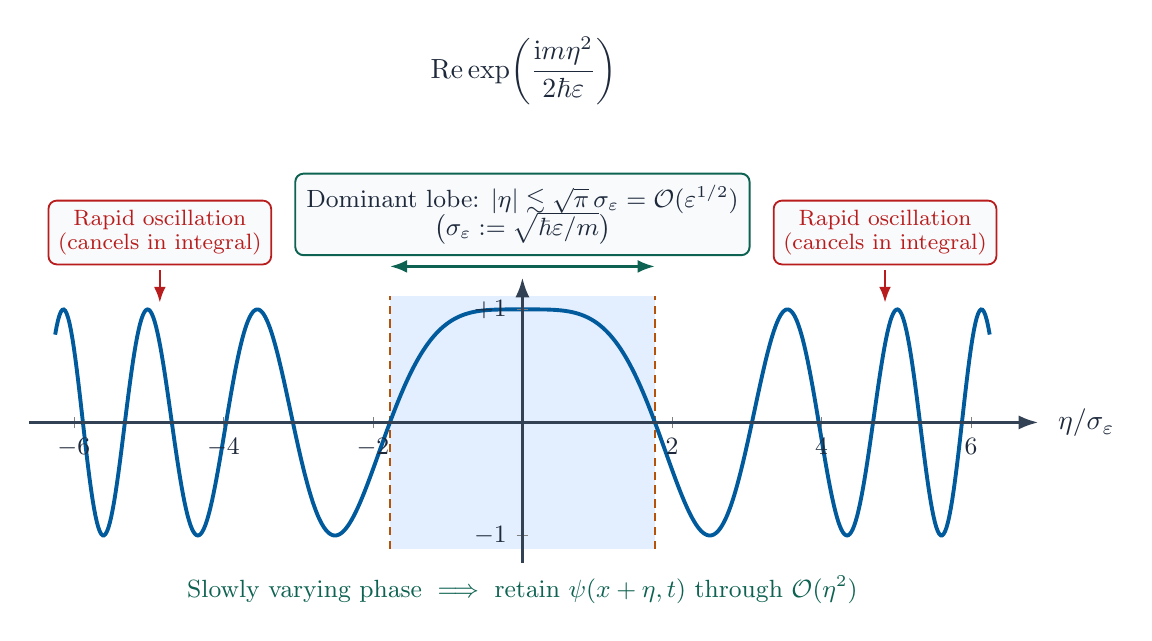
\begin{tikzpicture}[every node/.style={text=inkDark}]
    \begin{axis}[
        width=14.4cm,
        height=5.2cm,
        xmin=-6.6, xmax=6.9,
        ymin=-1.24, ymax=1.28,
        axis lines=middle,
        axis on top,
        axis line style={-{Latex[length=2.5mm,width=1.8mm]}, line width=0.95pt, draw=slateSub},
        xlabel={$\eta / \sigma_\varepsilon$},
        ylabel={$\operatorname{Re}\exp\!\left(\dfrac{\mathrm{i}m\eta^2}{2\hbar\varepsilon}\right)$},
        xlabel style={at={(axis description cs:1.01,0.49)}, anchor=west, font=\normalsize, text=inkDark},
        ylabel style={at={(axis description cs:0.49,1.03)}, anchor=south, font=\normalsize, text=inkDark, yshift=56pt},
        xtick={-6,-4,-2,2,4,6},
        xticklabels={$-6$,$-4$,$-2$,$2$,$4$,$6$},
        ytick={-1,1},
        yticklabels={$-1$,$+1$},
        tick label style={font=\small, text=inkDark},
        clip=false
    ]
        % Shaded central stationary lobe |u| <= sqrt(pi) ~ 1.7725
        \fill[bandBlue, opacity=0.78] (axis cs:-1.7725,-1.12) rectangle (axis cs:1.7725,1.12);
        \draw[accentAmber, line width=0.95pt, densely dashed] (axis cs:-1.7725,-1.12) -- (axis cs:-1.7725,1.12);
        \draw[accentAmber, line width=0.95pt, densely dashed] (axis cs:1.7725,-1.12) -- (axis cs:1.7725,1.12);

        % Exact Fresnel cosine curve cos(u^2 / 2)
        \addplot[
            domain=-6.25:6.25,
            samples=650,
            line width=1.4pt,
            draw=pathBlue
        ] {cos(deg(0.5*x*x))};

        % Central lobe width bracket cleanly above y-axis arrow (ymax=1.28)
        \draw[{Latex[length=2.2mm]}-{Latex[length=2.2mm]}, line width=1.0pt, draw=accentTeal]
            (axis cs:-1.7725, 1.38) -- (axis cs:1.7725, 1.38);

        % Central callout placed cleanly above the y-axis with ZERO line crossings
        \node[
            fill=boxFill, draw=accentTeal, line width=0.7pt, rounded corners=3pt,
            inner sep=4pt, font=\small, text=inkDark, align=center
        ] at (axis cs:0, 1.84)
            {Dominant lobe: $|\eta| \lesssim \sqrt{\pi}\,\sigma_\varepsilon = \mathcal{O}(\varepsilon^{1/2})$\\[-1pt]
             $\bigl(\sigma_\varepsilon := \sqrt{\hbar\varepsilon/m}\bigr)$};

        % Rapid oscillation annotations cleanly to left & right
        \node[
            fill=boxFill, draw=accentRed, line width=0.65pt, rounded corners=3pt,
            inner sep=3.5pt, font=\footnotesize, text=accentRed, align=center
        ] at (axis cs:-4.85, 1.68) {Rapid oscillation\\[-1pt] (cancels in integral)};
        \draw[-{Latex[length=2.0mm]}, draw=accentRed, line width=0.8pt]
            (axis cs:-4.85, 1.35) -- (axis cs:-4.85, 1.06);

        \node[
            fill=boxFill, draw=accentRed, line width=0.65pt, rounded corners=3pt,
            inner sep=3.5pt, font=\footnotesize, text=accentRed, align=center
        ] at (axis cs:4.85, 1.68) {Rapid oscillation\\[-1pt] (cancels in integral)};
        \draw[-{Latex[length=2.0mm]}, draw=accentRed, line width=0.8pt]
            (axis cs:4.85, 1.35) -- (axis cs:4.85, 1.06);

        % Bottom note cleanly below ymin=-1.24 with ZERO axis crossings
        \node[font=\small, text=accentTeal] at (axis cs:0, -1.48)
            {Slowly varying phase $\implies$ retain $\psi(x+\eta,t)$ through $\mathcal{O}(\eta^2)$};
    \end{axis}
\end{tikzpicture}
\end{document}
